\section{Supplemental Figures and Tables}

\begin{figure}[H]
	\centering
	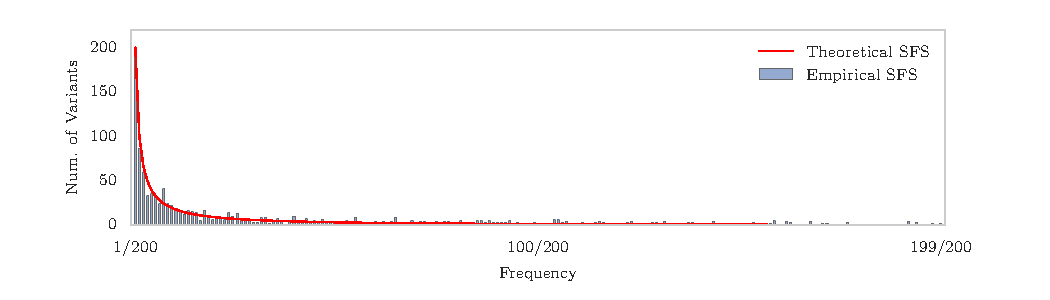
\includegraphics[trim=.01in 0.1in .01in 
	0.1in,clip,width=\textwidth]{figures/sfs.pdf}
	\caption{{\bf Site Frequency Spectrum.} Theoretical and
          Empirical SFS in a 50Kbp region for a neutral population of 200
          individuals when $N_e=10^6$ and $\mu=10^{-9}$. The $x$-axis 
          corresponds to site frequency, and
          the $y$-axis to the number of variants with a specific
          frequency. 
          In a neural population, majority of the variations stand in low 
          frequency.} \label{fig:sfs}
\end{figure}



\begin{figure}[H]
	\centering
	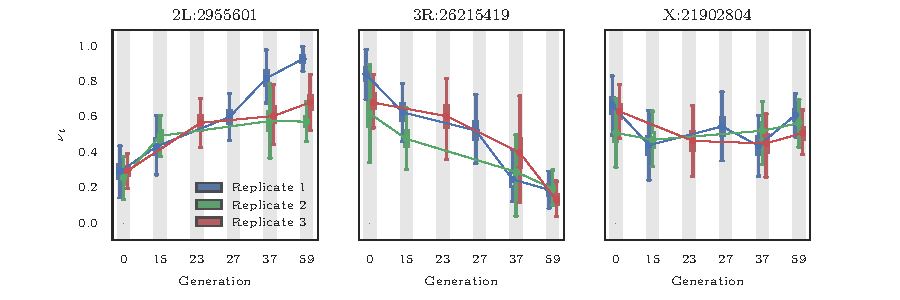
\includegraphics[width=\textwidth]{figures/trajectoryReal.pdf}
	\caption{{\bf Trajectory of pool-sequenced variants.}
          Trajectory of three different variants that are increasing
          in frequency over time. Note that for read count data, the
          true allele frequency is not known. Here we draw the
          posterior distribution of the allele frequency at each time
          point using box plot. The median of each distribution is
          denoted by dots. The variance of each box is seen to be
          inversely related to the depth of the measurement. For instance, 
          generation 59 is sequenced with higher coverage than generation 37. 
          As a result, variance of observations in generation 59 is 
          considerably 
          smaller.}
	\label{fig:trajectoryReal}
\end{figure}

\begin{figure}[H]
	\centering
	\includegraphics[trim=.0in 0 .0in 0, 
	clip,width=0.5\textwidth]{figures/{statePosterior}.pdf}
	\caption{{\bf Posterior distribution of allele frequency.}
          Distribution of hidden allele frequency for different values
          of depth $d=\{5,50,500\}$. In all cases, the true frequency
          is $0.2$. The estimated frequency values are binomially distributed, 
          with different variances,
          around the true value in all cases with.}
	\label{fig:stateConditional}
\end{figure}
\begin{figure}[H]
	\centering
	\begin{tabular}{c}
		\includegraphics[trim=.2in 0 .0in 0, 
		clip,width=\textwidth]{figures/{depthHetero}.pdf}
	\end{tabular}
	\caption{{\bf Coverage heterogeneity in time series data.} Each panel
          shows the read depth for 3
          replicates of the \datadm\ data (see section~\ref{sec:dmel}). 
          Heterogeneity in depth of coverage is 
          seen
          between replicates, and also at different time points, in
          all 4 variants. None of these sites pass the the hard filtering with 
          minimum depth of 30. }
	\label{fig:depthHetero}
\end{figure}

\begin{figure}[H]
	\centering 
	\includegraphics[width=\textwidth]{figures/{msmsts}.pdf}
	\caption{{\bf Dynamic SFS-based statistics.} Mean and 95\% CI
		of 100 simulations for neutral (blue trajectories) selection
		with $s=0.1$ (red trajectories). In all case, statistic computed for 
		a 50Kbp window and $N_e=10^4$, $\mu=10^{-9}$. The dashed line 
		shows 
		the parametric models derived in Appendix~\ref{app:td}.  }
	\label{fig:sfsts}
\end{figure}

\begin{figure}[H]
	\centering
	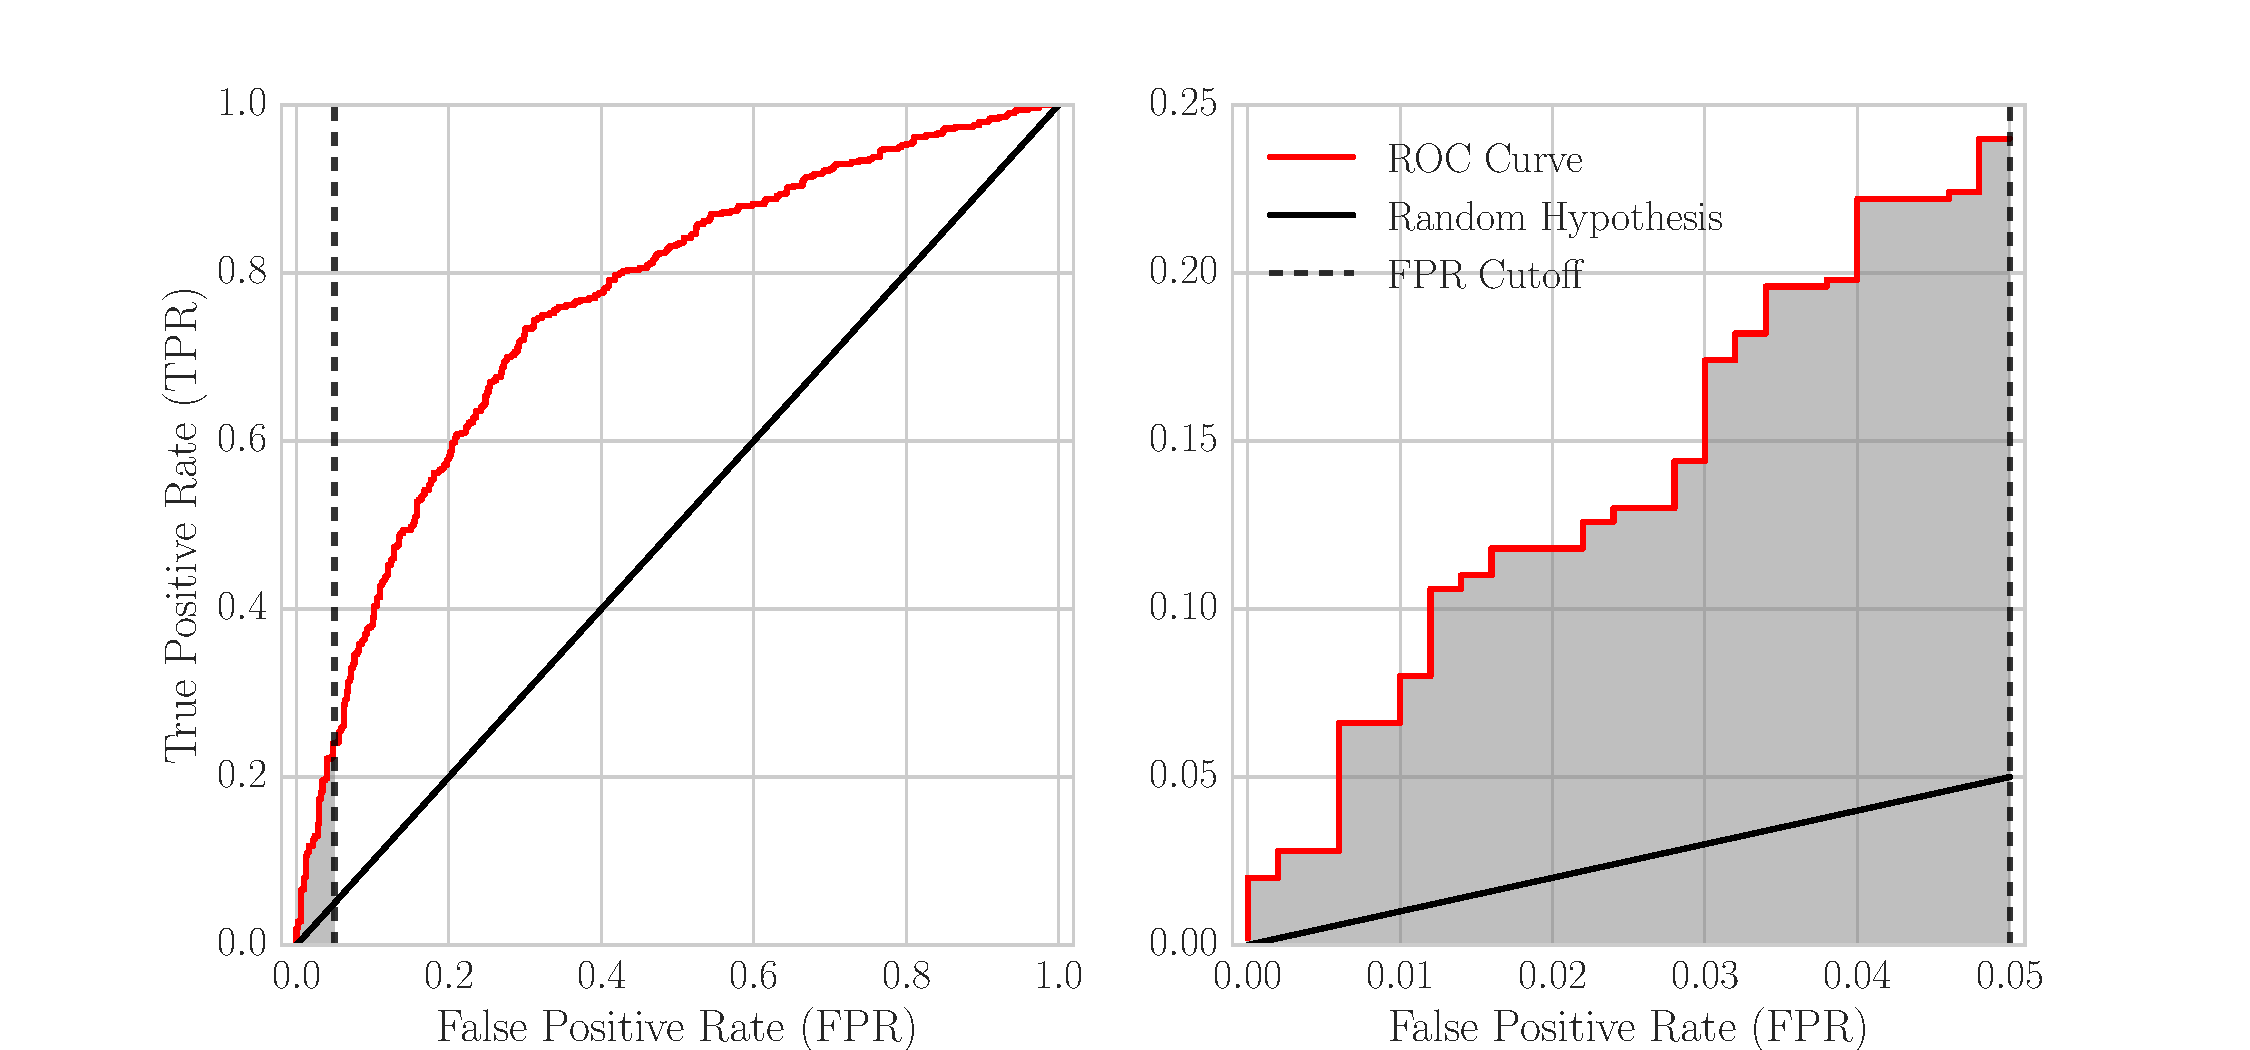
\includegraphics[trim=0.4in 0 .8in 0.02in , 
	clip,width=\textwidth]{figures/powerROC.pdf}
	\caption{{\bf Schematic for computing power of detecting
            selection.} Receiver Operating Characteristics (ROC) curve
            (left) for classification of 1,000 simulations (500 selection and
          500 neutral). The Area Under the Curve (AUC) represents
          overall performance. The diagonal black line represents
          performance of a random hypothesis which achieves Area under
          the curve (AUC) of 0.5. To avoid computing AUC for the
          regions where FPR is unacceptably high, we restrict ROC
          curve to the region where FPR$\le 0.05$ (right). In this
          case, we define power to be the (scaled) AUC of the
          restricted region.} \label{fig:powerROC}
\end{figure}






\begin{figure}[H]
	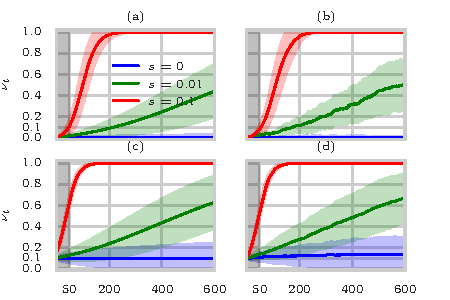
\includegraphics[trim=1in 0.1in 1in 
	0.1in,clip,width=\textwidth]{figures/AF.pdf}
	\caption{{\bf Theoretical (Markov chain) and Empirical
            trajectories of favored allele for hard and soft sweep
            scenarios}.  Theoretical (A,C) and empirical (B,D) trajectories of 
            the
          frequency of the favored allele are computed for $1000$ 
          simulations of populations with 
          $1000$ diploid individuals. Each curve shows the mean and the 95\% 
          confidence
          interval.  Panels A and C represent theoretical Markov chain
          based calculations of the favored allele frequency under
          hard ($\nu_0$ is small), and soft sweep due to standing
          variation (higher $\nu_0$), for a range of values of
          $s$. Note that $s=0$ corresponds to neutral
          evolution. Similarly, panels B and D show the empirical
          forward simulations of populations under the same selection
          regimes, and hard/soft-sweep scenarios. The first $50$
          generations are shaded in gray to represent the typical
          sampling span of EE experiments. The plot illustrates the
          difficulty of EE experiments in having to predict selection
          at a very early stage of the sweep. The signal is slightly
          stronger under standing variation scenario. The theoretical
          and empirical simulations are in close correspondence. }
	\label{fig:sweep}
\end{figure}

\begin{figure}[H]
	\centering
	\begin{tabular}{c}
		\includegraphics[trim=.2in 0 .0in 0, 
		clip,width=\textwidth]{figures/{depth}.pdf}
	\end{tabular}
	\caption{ {\bf Distribution of depth in the real data.}
		 Scaled PDF (A) and CDF (B) of the read depths of all ($\approx$20.1M) 
		 measurements, i.e., all replicates and time points of the all 
		 ($\approx$1.5M) variants.
		 Scaled PDF (C) and CDF (D) of the minimum depth of sites. While more 
		 than half 
		 most ($\approx$11.5M) of the measurements have depth of 50 or greater 
		 (dashed line in (A),(B)), only a small fraction ($\approx$10K) of 
		 variants (dashed line in (C),(D)) pass the filter of having minimum 
		 depth of 50.}  
	\label{fig:depth}
\end{figure}


\begin{figure}[H]
	\centering 
	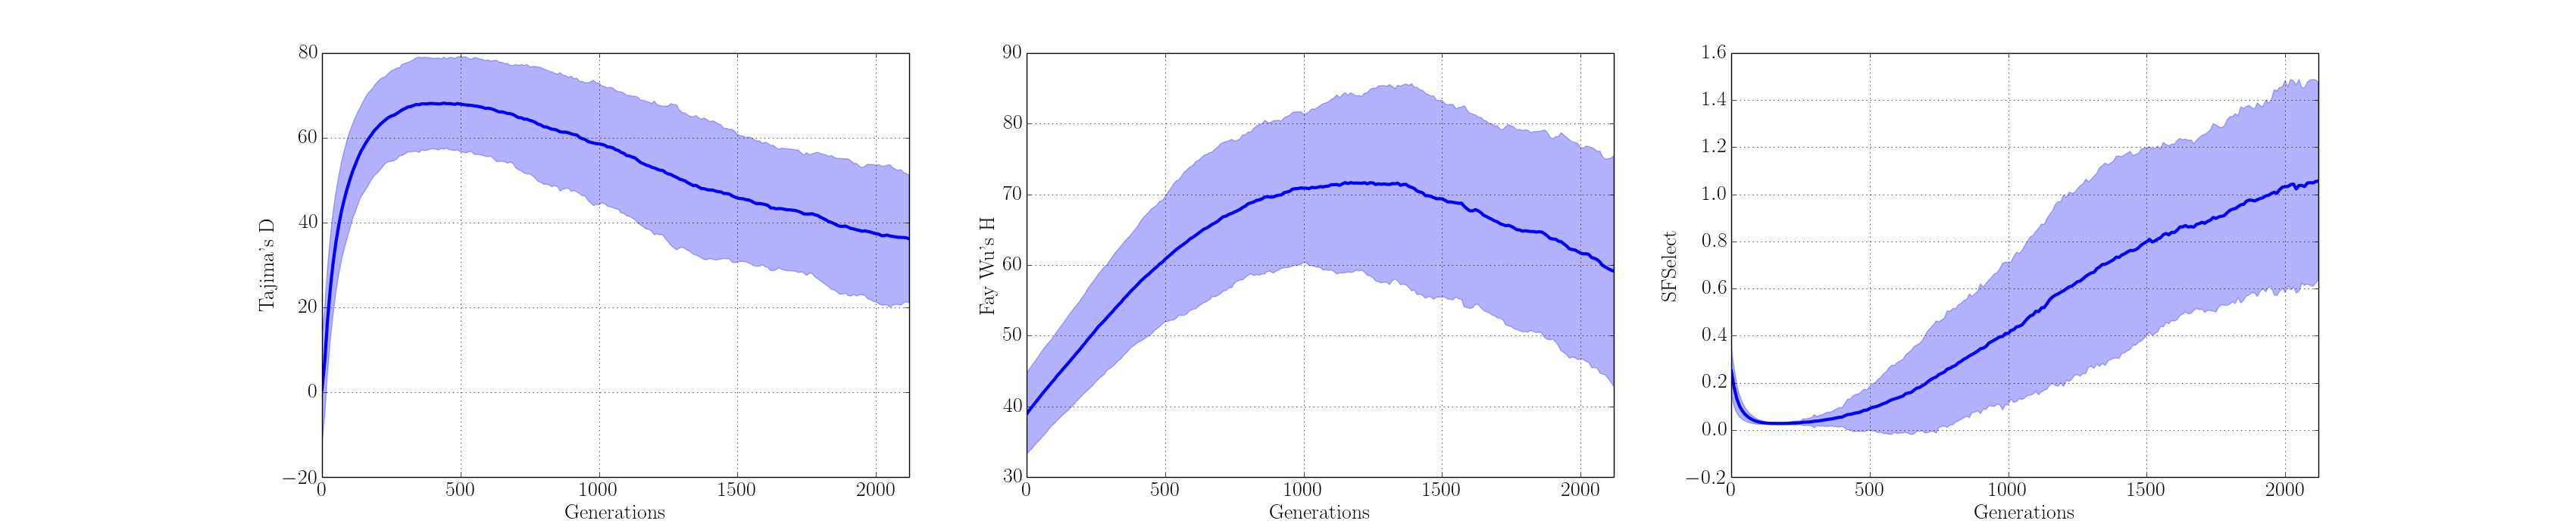
\includegraphics[trim=3.2in 0.1in 3.2in 0.2in , 
	clip,width=\textwidth]{figures/bottleneck}
	\caption{{\bf Effect of bottleneck in a typical experimental
			evolution experiment with restricted number of founder
			lines.} For the experiment, $F=200$ founders were selected
		from a larger population size ($N_e=10^{-6}$), and evolved
		under neutral scenario ($s=0$). The statistics for
		Tajima's $D$ (left), Fay Wu's $H$ (middle) and SFSelect were
		computed for 1000 neutral simulations and the mean and 95\%
		confidence interval plotted. Under neutral evolution, all
		the statistics are expected to vary around a fixed mean
		through time. However, under selective constraint, $D$ and
		$H$ take negative values, while SFSelect take positive
		values. In experimental evolution, bottleneck effect will
		suppress the signal of selection, especially in early
		generations. }
	\label{fig:bottleneck}
\end{figure}

\ignore{
\begin{figure}[H]
	\centering
	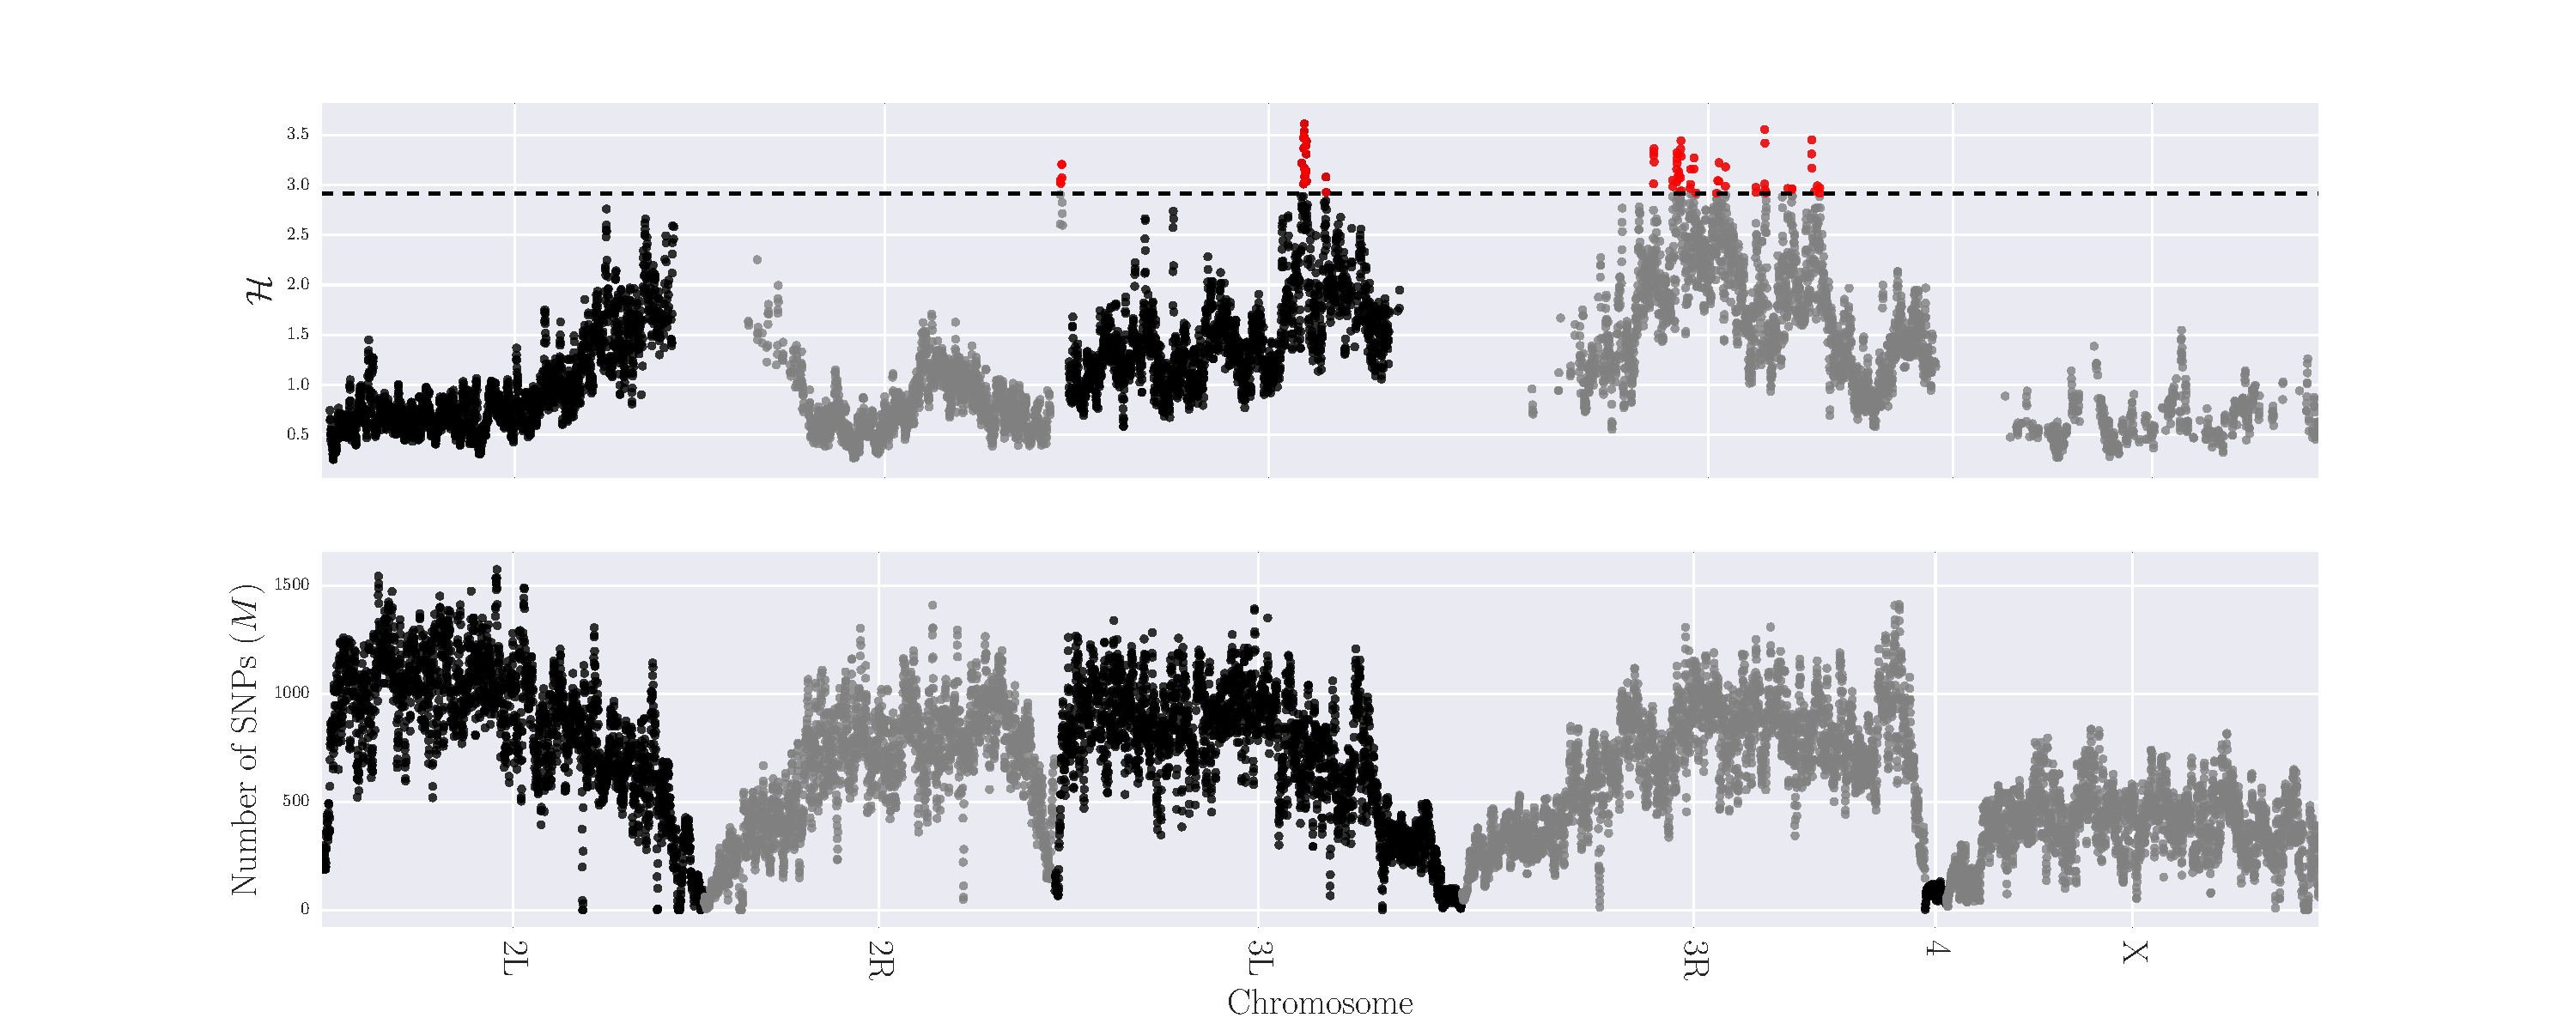
\includegraphics[width=\textwidth]{figures/manhattan.pdf}
	\caption{{\bf Manhattan plot.} Distribution of the composite $\Hc$ 
	statistic (top) 
		and the number of SNPs (bottom) for 50Kbp sliding window with steps of 
		10Kbp across genome. Regions in which their $\Hc$ statistic falls in 
		top one 
		percentile 
		distribution is denoted with red color. Pearson correlation between the 
		number of SNPs and 
		$\Hc$ of all windows is -0.03 and is -0.27 when restricting to the 
		candidate regions is -0.27. This 
		nine-fold increase in correlation implies that the $\Hc$ statistic 
		takes 
		more extreme values as the number of SNPs in the window is less than 
		expected ($\approx$1100). } 
	\label{fig:manhattan}
\end{figure}
}

\begin{figure}[H]
	\centering
	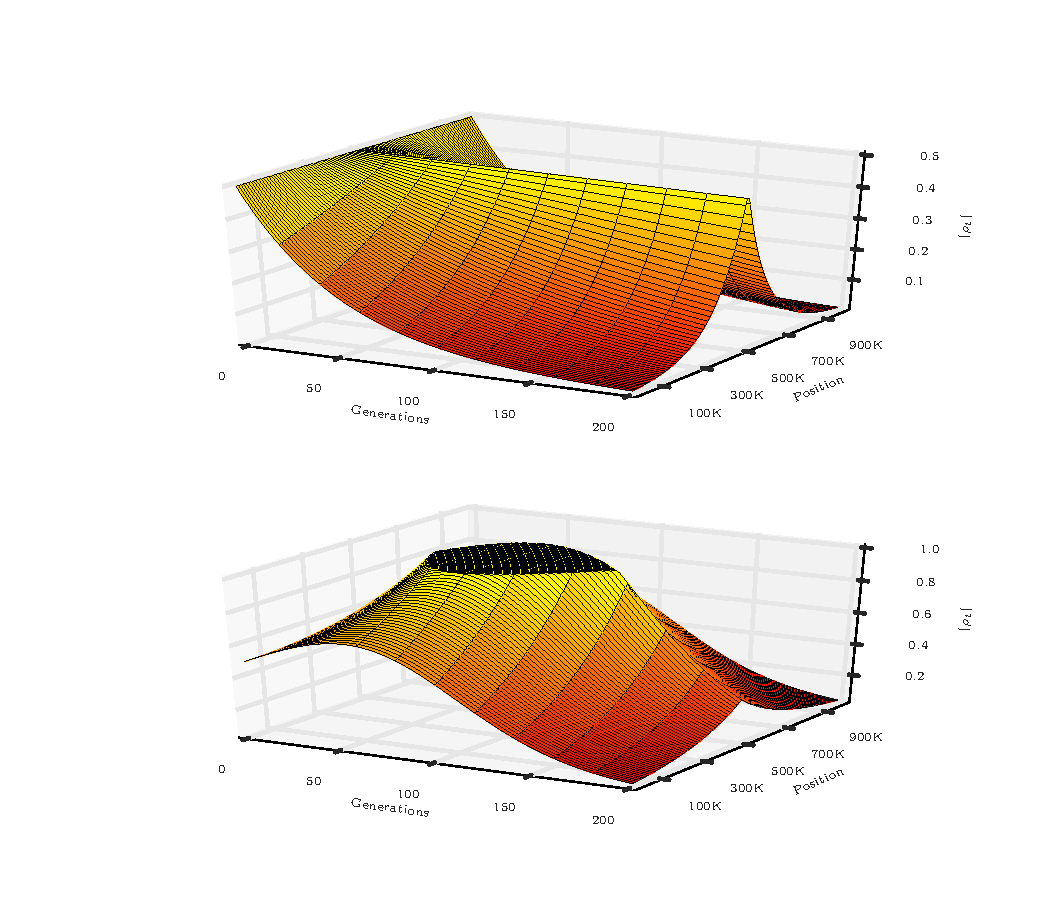
\includegraphics[width=\textwidth]{figures/LDDecay3d}
	\caption{ {\bf Expected dynamic of LD under selection and neutral 
	evolution.} Dynamic of LD ($\rho_t$) of a 1Mbp genome to the favored allele 
	(at position 500K) is drawn as function of position and time for neutral 
	(top) and selection(bottom) regimes.
	For sake of illustration, we assumed that at generations 0, LD of all 
	variants with the favored allele is 0.5, initial frequency of the favored 
	allele is 0.1, recombination rate is $r=2\times10^{-8}$ (top). The 
	selection strength is 0 and 0.05 for neutral and selection regimes, 
	respectively. As expected LD decay exponentially  through space and time. 
	However, selection causes LD to increase then decrease.}	
		\label{fig:ld3d}
\end{figure}

\begin{figure}[H]
	\centering
	\begin{tabular}{l|l}
		(A)&(B)\\
		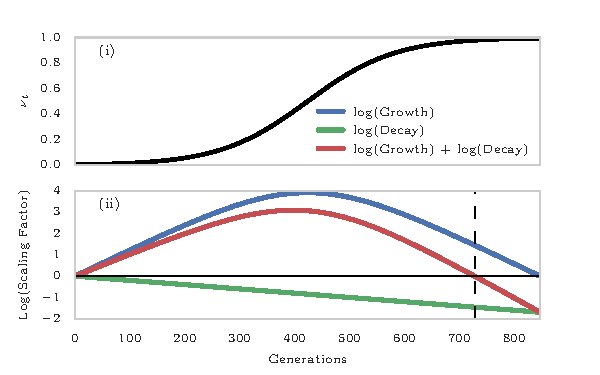
\includegraphics[width=0.5\textwidth]{figures/decayFactors0}
		&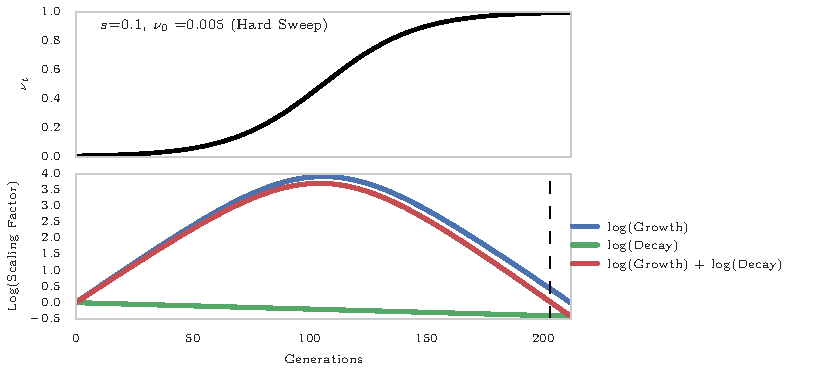
\includegraphics[width=0.5\textwidth]{figures/decayFactors1}\\
		\hline(C)&(D)\\
		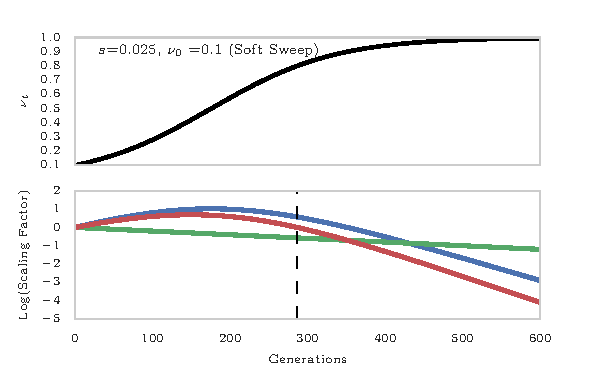
\includegraphics[width=0.5\textwidth]{figures/decayFactors2}
		&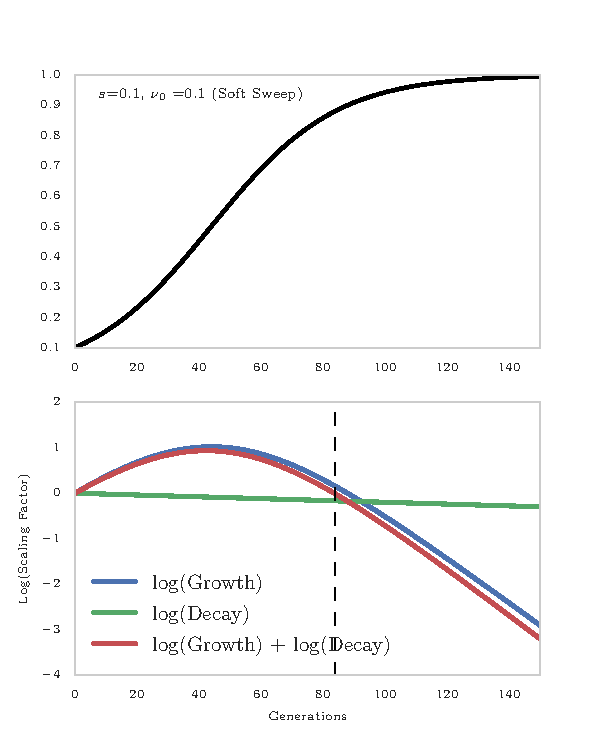
\includegraphics[width=0.5\textwidth]{figures/decayFactors3}		
	\end{tabular}
	
	\caption{{\bf Interaction between growth and decay factors of LD.}
		Expected evolution of LD under natural 
		selection for weak selection (s=$0.01$) and a distance of 100Kb between 
		sites for hard (A,B) and soft (C,D) sweeps. In addition to 
		recombination, initial frequency of the favored allele and selection 
		strength determine dynamic of LD. The vertical dashed line denotes the 
		time in which LD start to decrease. In all cases, LD increase in first 
		50 generations, which implies that localizing adaptive allele in short 
		term experimental evolution is a difficult task.} \label{fig:ldf}
\end{figure}



\begin{figure}[H]
	\centering
	\includegraphics[trim=.2in 0 .2in 0, 
	clip,width=\textwidth]{figures/{rank30.0}.pdf}
	\caption{{\bf Ranking performance for 30$\times$ coverage.}
           Cumulative Distribution Function (CDF) of the distribution
           of the rank of the favored allele in 500 simulations for
           \comale\ ($H$), Gaussian Process (GP), CMH, and Frequency
           Increment Test (FIT), for different values of selection
           coefficient $s$ and initial carrier frequency. Note that the
           individual variant \comale\ score ($H$) is used to rank
           variants.  The Area Under Curve (AUC) is computed as a
           quantitative measure to compare the performance of methods
           for each configuration.}
	\label{fig:rank30}
\end{figure}
\ignore{
\begin{figure}[H]
	\centering
	\includegraphics[trim=.2in 0 .2in 0, 
	clip,width=\textwidth]{figures/{rank300.0}.pdf}
	\caption{{\bf Ranking performance for 300$\times$ coverage.}
           Cumulative Distribution Function (CDF) of the distribution
           of the rank of the favored allele in 500 simulations for
           \comale\ ($H$), Gaussian Process (GP), CMH, and Frequency
           Increment Test (FIT), for different values of selection
           coefficient $s$ and initial carrier frequency. Note that the
           individual variant \comale\ score ($H$) is used to rank
           variants.  The Area Under Curve (AUC) is computed as a
           quantitative measure to compare the performance of methods
           for each configuration.}
	\label{fig:rank300}
\end{figure}}
\begin{figure}[H]
	\centering
	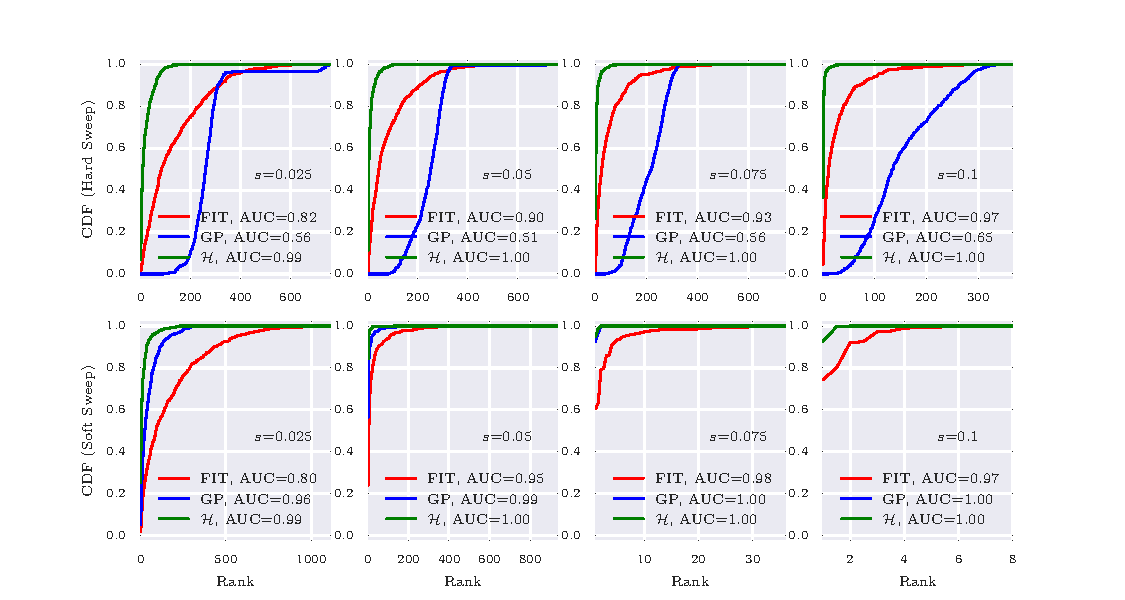
\includegraphics[trim=.2in 0 .2in 0, 
	clip,width=\textwidth]{figures/rankinf.pdf}
	\caption{{\bf Ranking performance for infinite coverage.}
           Cumulative Distribution Function (CDF) of the distribution
           of the rank of the favored allele in 500 simulations for
           \comale\ ($H$), Gaussian Process (GP), CMH, and Frequency
           Increment Test (FIT), for different values of selection
           coefficient $s$ and initial carrier frequency. Note that the
           individual variant \comale\ score ($H$) is used to rank
           variants.  The Area Under Curve (AUC) is computed as a
           quantitative measure to compare the performance of methods
           for each configuration.}
	\label{fig:rankinf}
\end{figure}


\begin{figure}[H]
	\centering
	\includegraphics[width=0.6\textwidth]{figures/{bias.30}.pdf}
	\caption{{\bf Distribution of bias for 30$\times$ coverage.} The
		distribution of bias ($s-\hat{s}$) in estimating selection
		coefficient over 500 simulations using Gaussian Process (GP) and
		\comale\ ($H$) is shown for a range of choices for the selection
		coefficient $s$ and starting carrier frequency $\nu_0$, when
		coverage $\lambda=30$ (Panels A,B). GP and \comale\ have similar
		variance in estimates of $s$ for soft sweep, while \comale\ provides
		lower variance in hard sweep. Also see Table~\ref{tab:biasdist}. Panels 
		C,D
		show the variance in the estimation of $h$.}
	\label{fig:bias30}
\end{figure}


\begin{figure}[H]
	\centering
	\includegraphics[width=0.6\textwidth]{figures/{bias.inf}.pdf}
	\caption{{\bf Distribution of bias for infinite coverage.} The
		distribution of bias ($s-\hat{s}$) in estimating selection
		coefficient over 500 simulations using Gaussian Process (GP) and
		\comale\ ($H$) is shown for a range of choices for the selection
		coefficient $s$ and starting carrier frequency $\nu_0$, when
		coverage $\lambda=\infty$ (Panels A,B). GP and \comale\ have similar
		variance in estimates of $s$ for soft sweep, while \comale\ provides
		lower variance in hard sweep. Also see Table~\ref{tab:biasdist}. Panels 
		C,D
		show the variance in the estimation of $h$.
		}
	\label{fig:biasinf}
\end{figure}


\begin{figure}[H]
	\centering
	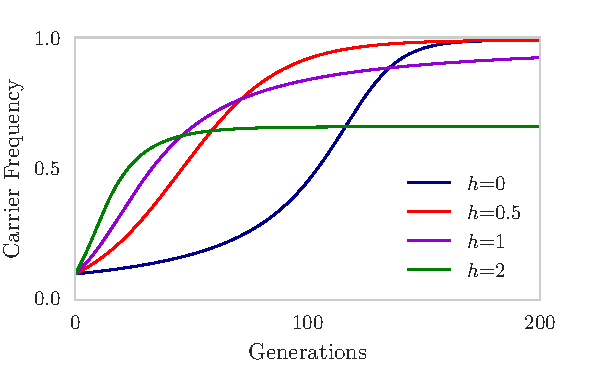
\includegraphics[width=0.8\textwidth]{figures/dominance.pdf}
	\caption{{\bf Natural selection in infinite population.} Trajectory of the 
	favored allele in an infinite population with $s=0.1$ for $h=0$ (recessive 
	favored allele), $h=0.5$ (directional selection), $h=1$ (dominant favored 
	allele) and $h=2$ (overdominant favored allele). }
	\label{fig:dominance}
\end{figure}

